\chapter{Selene: scripting interface}

\section{Principles}

\subsection{Organization}

Raytracing calculations are done by setting a scene up and feeding it to a renderer. This is first done by calling \lfc{MODE}(\lsg{selene}) which returns an instance of the Selene renderer. It only has a few functions that can modify it.

The first one is \lfc{N\_rays\_total}(\lin{N}) which will set the total number of rays that need to be computed.

Then the user has to define the optical elements, light sources, materials, etc, and feed them to the rendered. This is done by \lfc{add\_object}(\lud{object}) where \lud{object} is a Selene object, and \lfc{add\_light}(\lud{light}) where \lud{light} is a Selene light source.

Once this is done, the user needs to call \lfc{render}() to start the computation. This function can be called several times to run several simulations in a raw, after modifying an object's properties for instance.

Eventually, a typical script will look like
\begin{lstlisting}
sln=MODE("selene")
sln:N_rays_total(2000000)

% Scene definition

sln:add_object(object_1)
sln:add_object(object_2)
sln:add_light(source)

sln:render()
\end{lstlisting}

\subsection{Inner workings}

This is a summary of the rendering algorithm:

\begin{enumerate}
	\item At the beginning of the rendering the object and light sources locations are recomputed based on other objects. Various other properties can be computed, or memory or files allocated.
	\item A ray is created from one of the registered light sources and is fetched by renderer
	\item The intersection between this ray and every object is computed
		\begin{itemize}
			\item First, by computing the intersection with the bounding box first to have a quick approximation
			\item Then by computing the intersection with the various faces of the object, if the first step showed potential intersection
		\end{itemize}
	\item The intersections are looked through for the one with the smallest positive time, and the others are discarded
	\item The object related to that intersection is asked to treat the ray based on the face intersected and the intersection location
	\item It is determined from which side of the face (up or down, see \ref{faces_irfs}) the ray is coming
	\item The relevant Interface Response Function is given the ray and the refractive index of each side of the face, and determines how the ray must be redirected based or absorbed based on its optical properties
	\item Intersections for the new ray are computed again until it is either absorbed or lost
	\item The renderer fetches a new ray until the required number of rays has been computed
\end{enumerate}

\subsection{Probabilistic behavior}

\label{selene_probabilistic}
Raytracing usually follows a Monte-Carlo approach, that is to say one generates many random rays in a scene, and cast them with random directions and/or locations based on the properties of the sources, and have them intersect with objects.

How you handle those interactions, however, can be of two kinds: patch branching and probabilistic. To illustrate path branching, let's assume one computes the interaction of a ray with a glass surface. The transmission and reflection coefficients are not zero, so from one incident ray two would be generated. Those would then propagate again and generate new rays and so on. One can immediately notice that, in pathological cases, this could make the number of rays grow exponentially. Given enough computational time, it should be possible to address all of them, but then a lot of CPU time would have been spent computing the children of only one initial ray, giving much weight to that particular location.

With Selene, we have chosen to go with a full probabilistic approach. If an interface has a reflection, transmission, and absorption coefficient, energy conservation requires that
\begin{equation}
	R+T+A=1
\end{equation}
If one interprets this probabilistically, that means the sum of the probabilities for the ray to be reflected, transmitted or absorbed is 1. Another way to see it, is that one could split the numbers between 0 and 1 into three regions of lengths $R$, $T$ and $A$ as follows:
\begin{center}\begin{tikzpicture}
\draw [thick] (0,0) -- (10,0);
\draw [thick] (0,-0.5) -- (0,0.5);
\draw [thick] (10,-0.5) -- (10,0.5);
\draw [thick] (3,-0.5) -- (3,0.5);
\draw [thick] (8,-0.5) -- (8,0.5);
\draw (1.5,0) node[above]{$R$};
\draw (5.5,0) node[above]{$T$};
\draw (9,0) node[above]{$A$};
\draw (0,0.5) node[above]{0};
\draw (10,0.5) node[above]{1};
\draw [thick,-latex] (0,-1) -- (6,-1);
\draw (6,-1) node[right]{$p$};
\end{tikzpicture}\end{center}
if one takes a random number $p$ between 0 and 1, the region p falls in will determine the result of the calculation. This approach can be generalized to any number of effects the resulting ray could encounter. This ensures that one ray can only give rise to at most one ray.

While the probabilistic approach does not compute the exact behavior of a specific point, it will still statistically properly reconstruct the behavior of the whole neighborhood of it.

\subsection{Simulation summary}

After each call of \lfc{render} the program outputs a summary log under the file name \lsgnq{selene\_render\_X} within the \lfc{output\_directory}, where \lsgnq{X} is the render number, starting from 0. This file is a mini-script that specifies
\begin{itemize}
	\item the requested number of rays
	\item the power of each source
	\item the number of ray of each source
	\item the power carried by each ray
\end{itemize}

Its purpose is for the analysis of results after the render, for some of this information will be required.

\section{Relative positioning}

Selene's positioning system can be relative. That means objects can be placed relatively to others, or the world's origin of course.

\subsection{Orientation}

\label{selene_relative_positioning}
The first part of the positioning system is defining the object's orientation. Each object comes with its own frame, and most object primitives are aligned with a particular axis within this frame. For instance, the axis of a cylinder is aligned with the $\vec x$ axis of the object's frame. To rotate the cylinder in the world, one thus needs to rotate the frame itself.

This rotation is specified through Euler angles. The convention chosen in this software is yaw$\rightarrow$pitch$\rightarrow$roll, or $zy'x"$. That is, first the frame is rotated by an angle $\alpha$ around $\vec z$, then by an angle $\beta$ around the new $\vec y$ axis, and finally by an angle $\gamma$ around the new $\vec x$ axis.

\begin{center}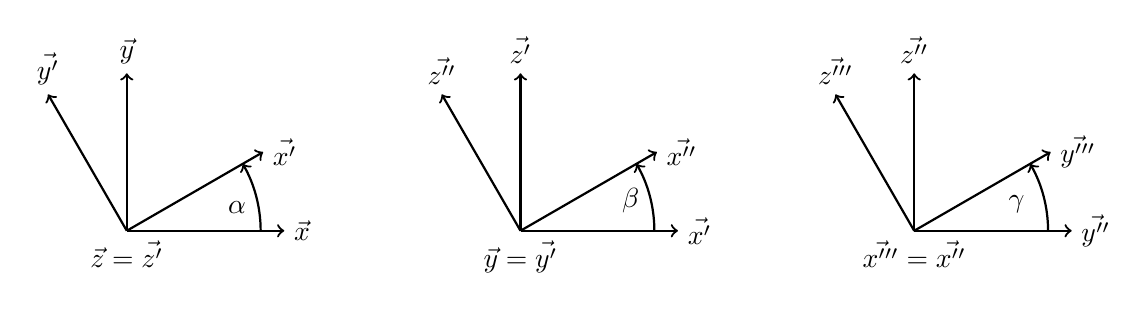
\begin{tikzpicture}
\draw [thick,->] (0,0) -- (2,0);
\draw [thick,->] (0,0) -- (0,2);
\draw (2,0) node[right]{$\vec{x}$};
\draw (0,2) node[above]{$\vec{y}$};
\draw (0,0) node[below]{$\vec{z}=\vec{z'}$};
\draw [thick,->](1.7,0) arc [start angle=0, end angle=30, radius=1.7];
\draw [thick,->] (0,0) -- (1.7321,1);
\draw [thick,->] (0,0) -- (-1,1.7321);
\draw (1.7321,1) node[right]{$\vec{x'}$};
\draw (-1,1.7321) node[above]{$\vec{y'}$};
\draw (1.4,0.1) node[above]{$\alpha$};

\draw [thick,->] (5,0) -- (7,0);
\draw [thick,->] (5,0) -- (5,2);
\draw (7,0) node[right]{$\vec{x'}$};
\draw (5,2) node[above]{$\vec{z'}$};
\draw (5,0) node[below]{$\vec{y}=\vec{y'}$};
\draw [thick,->](6.7,0) arc [start angle=0, end angle=30, radius=1.7];
\draw [thick,->] (5,0) -- (6.7321,1);
\draw [thick,->] (5,0) -- (4,1.7321);
\draw (6.7321,1) node[right]{$\vec{x''}$};
\draw (4,1.7321) node[above]{$\vec{z''}$};
\draw (6.4,0.1) node[above]{$\beta$};

\draw [thick,->] (10,0) -- (12,0);
\draw [thick,->] (10,0) -- (10,2);
\draw (12,0) node[right]{$\vec{y''}$};
\draw (10,2) node[above]{$\vec{z''}$};
\draw (10,0) node[below]{$\vec{x'''}=\vec{x''}$};
\draw [thick,->](11.7,0) arc [start angle=0, end angle=30, radius=1.7];
\draw [thick,->] (10,0) -- (11.7321,1);
\draw [thick,->] (10,0) -- (9,1.7321);
\draw (11.7321,1) node[right]{$\vec{y'''}$};
\draw (9,1.7321) node[above]{$\vec{z'''}$};
\draw (11.3,0.1) node[above]{$\gamma$};
\end{tikzpicture}\end{center}

 Now, this rotation can either be absolute, or relative to another object. In the latter case, the reference rotation frame will need to be set through the \lfc{rotation\_frame}(\lud{object}) function. The frame of the object we want to manipulate will be set identical to the frame of the reference, and then rotated.

\subsection{Placement}

The second part of the system is relative locations. Once an objet's orientation is set, it can be placed in the scene relatively to the world's origin or to another object. The purpose is to define object groups that can move with eachother. Now, this relative location does not necessarily need to be defined from an object's origin to another's. Indeed, some objects have particular points of interest, and it can be useful to place objects relatively to those points. For instance, two lenses can be aligned so that their focal points match. In this case, the relative locations of the lenses' centers is irrelevant. Those points will be called anchors, and each object type will have its own anchors depending on its parameters.

The process is illustrated with the figure below.
\begin{center}
\begin{tikzpicture}[scale=2.5]
\draw (0,0) node[below left]{O$_1$};
\draw [thick,->] (-0.5,0) -- (1,0);
\draw [thick,->] (0,-0.5) -- (0,1);
\draw (1,0) node[below]{$\vec{x_1}$};
\draw (0,1) node[left]{$\vec{y_1}$};
\draw (1.1,0.8) -- (1.3,0.8);
\draw (1.2,0.7) -- (1.2,0.9);
\draw (1.2,0.8) node[below]{A};
\draw [red,thick,->] (0.767,1.05) -- (2.066,0.3);
\draw [red,thick,->] (0.95,0.367) -- (1.7,1.666);
\draw (2.0666,0.3) node[red,below]{$\vec{x_D}$};
\draw (1.7,1.666) node[red,above left]{$\vec{y_D}$};
\draw [blue] (2.9,2) -- (3.1,2);
\draw [blue] (3,1.9) -- (3,2.1);
\draw (3,2) node[blue,above left]{B};
\draw [dgreen,thick,->] (1.2,0.8) -- (3,2);
\draw (2.1,1.4) node[dgreen,below]{$\vec{D}$};
\draw [blue,thick,->] (3.35,1.933) -- (4.1,0.634);
\draw [blue,thick,->] (3.167,1.25) -- (4.466,2);
\draw (3.6,1.5) node[blue,below]{O$_2$};
\draw (4.1,0.634) node[blue,right]{$\vec{x_2}$};
\draw (4.466,2) node[blue,right]{$\vec{y_2}$};
\end{tikzpicture}\end{center}
In this, we have two objects O$_1$ and O$_2$. First, O$_2$ had its orientation set, which is different from O$_1$'s orientation. O$_1$ has an anchor A, and O$_2$ an anchor B, and we want both anchors to be displaced relatively to eachother through the vector $\vec D$. Moreover, $\vec D$ itself can be expressed in a frame that is independent from O$_1$ and O$_2$. We will then define the following properties for O$_2$:
\begin{itemize}
	\item B will be its new origin
	\item A, belonging to O$_1$, will be set as its displacement reference.
	\item the frame D will be set based on any other frame in the scene, and $\vec D$ will be defined within it
\end{itemize}	
We will then have
\begin{equation}
	\vec{O_2}=\vec{O_1}+\vec{O_1 A} + \vec D+\vec{B O_2}
\end{equation}

\section{Faces and Interface Response Functions}

\label{faces_irfs}

\subsection{Face orientation}

\subsubsection{Up and Down}

The core elements with which rays in Selene interact are the faces of the various objects of a scene, and this section aims to describes what happens.

Faces come in favious shapes. They can be a plane, a parabola, a triangle, etc. In every case, faces have two sides, and the software is made so that do not necessarily behave the same sway. We thus need to be able to differentiate both sides, and this is done by the orientation of the normal vector to a face.

The direction towards which the normal vector is pointing will be known as ``up'', or the outside of a closed surface, and the opposite direction will be known as ``down'', or the inside of a closed surface.
\begin{figure}[!ht]
\begin{center}\begin{tikzpicture}[decoration={markings,mark= at position 0.5 with {\arrow{stealth}}}]
\draw (0,4) .. controls (2,3) and (4,1) .. (3,0);
\draw (0.5,4) node[right]{Face};
\draw (0,0) node[right]{Down/Inside};
\draw (4,0) node[right]{Up/Outside};
\draw [ thick,-latex] (2.95,1.56) -- (5.5,3.2);
\draw (4.225,2.38) node[below right,text width=2cm]{Normal Vector};
\draw [very thick,-,blue,postaction={decorate}] (1,2.1) -- (2.95,1.56);
\draw (2.95,1.56) node[blue,below left,text width=2cm]{Ray going outside};
\draw [very thick,-,red,postaction={decorate}] (2.5,3.5) -- (2.95,1.56);
\draw (2.5,3.5) node[red,above right]{Ray going inside};
\end{tikzpicture}\end{center}
\caption{Conventions around faces in Selene}
\end{figure}
The direction of the normal vector determines how an incident ray will interact with the face. If the scalar product between the direction vector of a ray and the normal factor of the face is positive, then the ray is going outside, and will be treated using the ``down'' properties of the face. If that scalar product is negative, the ray is going inside, and will be treated using the ``up'' properties.

\subsubsection{Properties of each side}

The most obvious property difference between the up and down sides is the material they refer to. After all, faces are supposed to represent where there is a change in refractive index. As such, each side will point to a different material defined by the user. Note that in some cases, like a transparent sensor surface that is not supposed to modify rays, the materials of both sides can be the same.

But merely knowing the materials is not enough to define what will happen to an incident ray. Indeed, while one could just use them to compute refraction and reflection, this is not the only way a surface can behave. Photons can be scattered, diffracted, absorbed, etc. To handle those different behaviors, we use what we call an Interface Response Function, or IRF. The purpose of the IRF will be to redirect a ray or destroy it depending of the various properties of the face.

We've chosen to make it so that both sides of a face don't necessarily have the same IRF. It can be used to define non-physical, but convenient, behaviors such as a face being perfectly antireflective from one side, and perfectly reflective from the other, or to input simulation data for both sides (the behavior of nanostructures for  instance will not be perfectly symmetrical). As such, both sides will refer to a potentially different IRFs.

Certains IRFs will require complete frames to determine the direction of the outgoing ray. In the case of Snell's law such a frame can be determined from the normal vector and the ray direction alone, but this would not work with a diffraction grating. As such, faces have an additional properties: a tangent vector. This vector is specified per face, per side, and can be fixed or have a special configuration that will adapt to the face. More details are to be found in the objects descriptions.

\subsection{The Interface Response Function}

As stated before, the purpose of the Interface Response Function is to turn an incident ray into a reflected or transmitted ray, or to absorb it, in the manner described in section \ref{selene_probabilistic}. This this done in accordance to the refractive index of the related face and its tangent vector.

To each specific optical behavior corresponds an IRF. See the section \ref{selene_object_funcs} to known how to assign them to objects.

\subsubsection{Default IRFs}

There are several default, basic IRFs, than can be passed to objects. They are
\begin{itemize}
	\item[] \textbf{SEL\_IRF\_FRESNEL}: the interface's response obeys the Fresnel coefficients of the associated materials, while the 
	\item[] \textbf{SEL\_IRF\_PERFECT\_ABSORBER}: all rays hitting the interface are absorbed and disappear
	\item[] \textbf{SEL\_IRF\_PERFECT\_ANTIREFLECTOR}: all rays hitting an interface go through it, but still obey Snell's law
	\item[] \textbf{SEL\_IRF\_PERFECT\_MIRROR}: rays are always reflected
\end{itemize}

\subsubsection{User defined IRFs}

\newpage
\section{Objects}

Selene objects are added through the function \lfc{Selene\_object}(\lsg{type},\lft{args}). Here, \lft{args} is actually a variable sequence of argument depending on the object \lud{type}. For instance, a sphere will only have one possible argument, its radius, while a cylinder will have two: its length and radius. This function returns an object which can then be manipulated in the script (see \ref{selene_object_funcs}).

\noindent Usage example:
\begin{lstlisting}
obj=Selene_object("cylinder",0.5,5.0)
\end{lstlisting}

\subsection{Functions common to all objects}

\label{selene_object_funcs}
%\addtocontents{toc}{\protect\setcounter{tocdepth}{2}}

\subsubsection[contains]{\lfc{contains}(\lft{x},\lft{y},\lft{z})}

Returns 1 if the object contains the point defined by $(x,y,z)$, and zero otherwise. Only valid for volume objects. It can still be called with the others but will return an undefined value.
\begin{lstlisting}
var=obj:contains(0.25,0,1.5)
\end{lstlisting}

\subsubsection[default\_in\_IRF]{\lfc{default\_in\_IRF}(\lud{IRF})}

Sets the IRF for every face of the object, on the down side, to \lud{IRF}.
\begin{lstlisting}
obj:default_in_IRF(SEL_IRF_PERFECT_ABSORBER)
\end{lstlisting}

\subsubsection[default\_in\_mat]{\lfc{default\_in\_mat}(\lud{Material})}

Sets the material for every face of the object, on the down side, to \lud{Material}.
\begin{lstlisting}
obj:default_in_mat(Glass)
\end{lstlisting}

\subsubsection[default\_IRF]{\lfc{default\_IRF}(\lud{IRF})}

Sets the IRF for every face of the object, on the both sides, to \lud{IRF}.
\begin{lstlisting}
obj:default_IRF(SEL_IRF_FRESNEL)
\end{lstlisting}

\subsubsection[default\_out\_IRF]{\lfc{default\_out\_IRF}(\lud{IRF})}

Sets the IRF for every face of the object, on the up side, to \lud{IRF}.
\begin{lstlisting}
obj:default_out_IRF(SEL_IRF_PERFECT_MIRROR)
\end{lstlisting}

\subsubsection[default\_out\_mat]{\lfc{default\_out\_mat}(\lud{Material})}

Sets the material for every face of the object, on the up side, to \lud{Material}.
\begin{lstlisting}
obj:default_out_mat(Air)
\end{lstlisting}

\subsubsection[face\_down\_IRF]{\lfc{face\_down\_IRF}(\lin{face number},\lud{IRF})}

Sets the down IRF of the face indexed by \lin{face number} (starting at 0) to \lud{IRF}.
\begin{lstlisting}
obj:face_down_IRF(0,SEL_IRF_PERFECT_ANTIREFLECTOR)
\end{lstlisting}

\subsubsection[face\_down\_mat]{\lfc{face\_down\_mat}(\lin{face number},\lud{Material})}

Sets the down material of the face indexed by \lin{face number} (starting at 0) to \lud{Material}.
\begin{lstlisting}
obj:face_down_mat(12,sapphire)
\end{lstlisting}

\subsubsection[face\_down\_tangent (two arguments)]{\lfc{face\_down\_tangent}(\lin{face number},\lsg{type})}

Sets type of the down tangent of the face indexed by \lin{face number} (starting at 0) to \lsgnq{type}. See the objects properties for more details.
\begin{lstlisting}
obj:face_down_tangent(4,"polar")
\end{lstlisting}

\subsubsection[face\_down\_tangent (four arguments)]{\lfc{face\_down\_tangent}(\lin{face number},\lft{x},\lft{y},\lft{z})}

Sets =the down tangent of the face indexed by \lin{face number} to the vector (\lft{x},\lft{y},\lft{z}).
\begin{lstlisting}
obj:face_down_tangent(0,1,0,0)
\end{lstlisting}

\subsubsection[face\_IRF]{\lfc{face\_IRF}(\lin{face number},\lud{IRF})}

Sets the IRF of the face indexed by \lin{face number} (starting at 0), on both sides, to \lud{IRF}.
\begin{lstlisting}
obj:face_IRF(0,SEL_IRF_FRESNEL)
\end{lstlisting}

\subsubsection[face\_up\_IRF]{\lfc{face\_up\_IRF}(\lin{face number},\lud{IRF})}

Sets the up IRF of the face indexed by \lin{face number} (starting at 0) to \lud{IRF}.
\begin{lstlisting}
obj:face_up_IRF(2,SEL_IRF_PERFECT_ANTIREFLECTOR)
\end{lstlisting}

\subsubsection[face\_up\_mat]{\lfc{face\_up\_mat}(\lin{face number},\lud{Material})}

Sets the up material of the face indexed by \lin{face number} (starting at 0) to \lud{Material}.
\begin{lstlisting}
obj:face_up_mat(1,Air)
\end{lstlisting}

\subsubsection[face\_up\_tangent (two arguments)]{\lfc{face\_up\_tangent}(\lin{face number},\lsg{type})}

Sets type of the up tangent of the face indexed by \lin{face number} (starting at 0) to \lsgnq{type}. See the objects properties for more details.
\begin{lstlisting}
obj:face_up_tangent(2,"polar_neg")
\end{lstlisting}

\subsubsection[face\_up\_tangent (four arguments)]{\lfc{face\_up\_tangent}(\lin{face number},\lft{x},\lft{y},\lft{z})}

Sets the up tangent of the face indexed by \lin{face number} to the vector (\lft{x},\lft{y},\lft{z}).
\begin{lstlisting}
obj:face_up_tangent(4,0,1,0)
\end{lstlisting}

\subsubsection[location]{\lfc{location}(\lft{x},\lft{y},\lft{z})}

Sets the object location to (\lft{x},\lft{y},\lft{z}) within the translation frame. The true location will be defined according to the relative positioning system. See \ref{selene_relative_positioning} for a detailled explanation.
\begin{lstlisting}
obj:location(1,1,0)
\end{lstlisting}

\subsubsection[name]{\lfc{name}(\lsg{object name})}

Sets the object name to \lsgnq{name}.
\begin{lstlisting}
obj:name("main_lens")
\end{lstlisting}

\subsubsection[origin]{\lfc{origin}(\lsgnq{anchor name})}

Sets the origin of the object to its anchor defined by \lsgnq{anchor name}. See \ref{selene_relative_positioning} for more details, and the objects descriptions for a list of the anchors.
\begin{lstlisting}
obj:origin(SEL_OBJ_BOX_FACE_XP)
\end{lstlisting}

\subsubsection[relative\_origin]{\lfc{relative\_origin}(\lud{relative frame},\lsgnq{anchor name})}

Sets the relative origin of the object to anchor of the \lud{relative frame} designed by \lsgnq{anchor name}. See \ref{selene_relative_positioning} for more details, and the objects descriptions for a list of the anchors.
\begin{lstlisting}
obj:relative_origin(object_0,SEL_OBJ_BOX_CORNER_XM_YM_ZM)
\end{lstlisting}

\subsubsection[rotation]{\lfc{rotation}(\lft{$\alpha$},\lft{$\beta$},\lft{$\gamma$})}

Set the angles of rotation of the object to \lft{$\alpha$}, \lft{$\beta$} and \lft{$\gamma$}, in degrees, relative to the \lud{rotation frame}. See \ref{selene_relative_positioning} for more details.
\begin{lstlisting}
obj:rotation(45,20,0)
\end{lstlisting}

\subsubsection[rotation\_frame]{\lfc{rotation\_frame}(\lud{frame})}

Set the relative rotation frame of the object the to one held by \lud{frame}. See \ref{selene_relative_positioning} for more details.
\begin{lstlisting}
obj:rotation_frame(object_1)
\end{lstlisting}

\subsubsection[translation\_frame]{\lfc{translation\_frame}(\lud{frame})}

Set the relative translation frame of the object to the one held by \lud{frame}. See \ref{selene_relative_positioning} for more details.
\begin{lstlisting}
obj:translation_frame(object_0)
\end{lstlisting}

\subsubsection[sensor]{\lfc{sensor}(\lsg{transp}/\lsg{abs},\lsg{options 1},\lsg{options 2},...)}

Will turn the object into a sensor. See the section \ref{selene_sensors} for a full description of the options and what they do.
\begin{lstlisting}
obj:sensor("abs","wavelength","ID","obj_intersection")
\end{lstlisting}

\newpage
\subsection{Volume primitives}

Volume objects are objects that are defined by a closed surface.

\subsubsection{Box}

As its name indicates, the \lud{box} object is just a block with parallel faces, over variable width, heights and length. As such, adding one in the script will involve \lfc{Selene\_object}(\lsg{box},\lft{lx},\lft{ly},\lft{lz}), where \lft{lx} and so on will be the length along the $x$, $y$ and $z$ axes. By default, the box' origin is its center, meaning it extends from $-lx/2$ to $+lx/2$, and so on.

\noindent Example:
\begin{lstlisting}
obj=Selene_object("box",2,3,4)
\end{lstlisting}

The default anchor is the center of the \lud{box}: SEL\_OBJ\_BOX\_CENTER

However, the following specific point serve as anchors for the \lud{box} object. Here, XM refers to the first face on the $x$ axis, and XP refers to the second face on the $x$ axis. The same goes for the $y$ and $z$ axes. There are six face anchors corresponding to the center of each face, and eight corner anchors corresponding to each vertex of the box.

\begin{tabular}{|c|c|}
\hline
Faces & Corners \\
\hline
SEL\_OBJ\_BOX\_FACE\_XM & SEL\_OBJ\_BOX\_CORNER\_XM\_YM\_ZM \\
SEL\_OBJ\_BOX\_FACE\_XP & SEL\_OBJ\_BOX\_CORNER\_XP\_YM\_ZM \\
SEL\_OBJ\_BOX\_FACE\_YM & SEL\_OBJ\_BOX\_CORNER\_XM\_YP\_ZM \\
SEL\_OBJ\_BOX\_FACE\_YP & SEL\_OBJ\_BOX\_CORNER\_XP\_YP\_ZM \\
SEL\_OBJ\_BOX\_FACE\_ZM & SEL\_OBJ\_BOX\_CORNER\_XM\_YM\_ZP \\
SEL\_OBJ\_BOX\_FACE\_ZP & SEL\_OBJ\_BOX\_CORNER\_XP\_YM\_ZP \\
& SEL\_OBJ\_BOX\_CORNER\_XM\_YP\_ZP \\
& SEL\_OBJ\_BOX\_CORNER\_XP\_YP\_ZP \\
\hline
\end{tabular}


\newpage
\subsubsection{Cone}

\begin{itemize}
	\item \textbf{SEL\_OBJ\_CONE\_CENTER}
	\item \textbf{SEL\_OBJ\_CONE\_FACE}
	\item \textbf{SEL\_OBJ\_CONE\_TIP}
\end{itemize}

\newpage
\subsubsection{Cylinder}

\begin{center}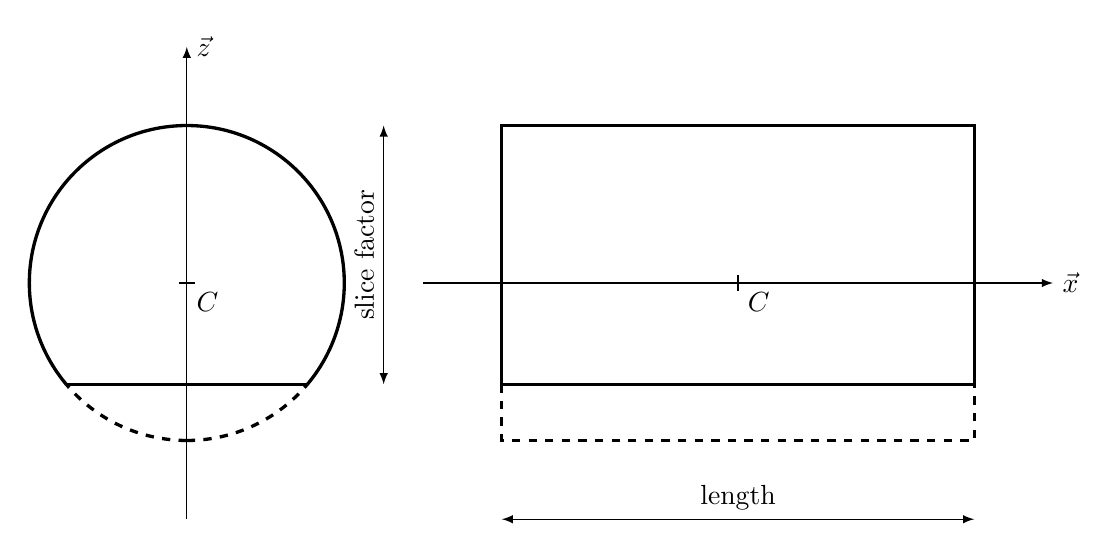
\begin{tikzpicture}
\draw [-latex] (0,-3) -- (0,3);
\draw (0,3) node[right]{$\vec{z}$};
\draw [-] (-0.1,0) -- (0.1,0);
\draw (0,0) node[below right]{$C$};

\draw [very thick,-](0,2) arc [start angle=90, end angle=220, radius=2];
\draw [very thick,-](0,2) arc [start angle=90, end angle=-40, radius=2];
\draw [very thick,dashed](0,-2) arc [start angle=-90, end angle=-140, radius=2];
\draw [very thick,dashed](0,-2) arc [start angle=-90, end angle=-40, radius=2];
\draw [very thick,-] (-1.5321,-1.2856) -- (1.5321,-1.2856);

\draw [latex-latex] (2.5,-1.2856) -- (2.5,2) node [midway,above,sloped] {slice factor};

\draw [-latex] (3,0) -- (11,0);
\draw (11,0) node[right]{$\vec{x}$};
\draw [very thick] (4,-1.2856) rectangle (10,2);
\draw [very thick,dashed] (4,-1.2856) -- (4,-2) -- (10,-2) -- (10,-1.2856);
\draw [-] (7,-0.1) -- (7,0.1);
\draw (7,0) node[below right]{$C$};
\draw [latex-latex] (4,-3) -- (10,-3) node [above,midway] {length};
\end{tikzpicture}\end{center}

The anchor points are
\begin{itemize}
	\item \textbf{SEL\_OBJ\_CYL\_CENTER} : the cylinder center
	\item \textbf{SEL\_OBJ\_CYL\_FACE\_XM} : the center of the face first intersecting the $x$ axis
	\item \textbf{SEL\_OBJ\_CYL\_FACE\_XP} : the center of the face last intersecting the $x$ axis
\end{itemize}

\newpage
\subsubsection{Lens}

While lenses could be defined from a sequence of spherical patches, a volume lens primitive is provided through the function \lfc{Selene\_object}(\lsg{lens},\lft{thickness},\lft{radius},\lft{$r_1$},\lft{$r_2$}).

A lens is made of two spherical caps and one cylinder. \lft{thickness} specifies the intersection points of each cap with the $\vec x$ axis of the lens, the first one being at -\lft{thickness}/2 and the second at \lft{thickness}/2. \lft{$r_1$} and \lft{$r_2$} are the radii of each, and \lft{radius} is the maxiùam radius of the lens from its axis.
\begin{center}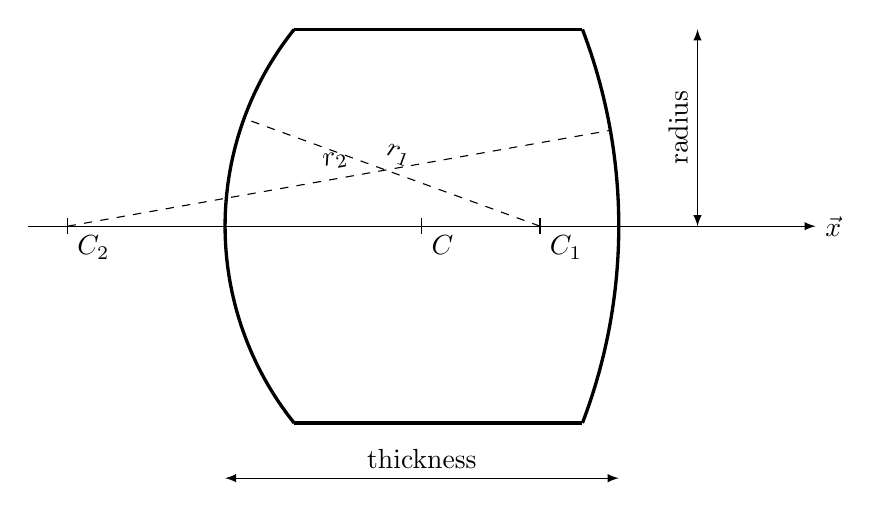
\begin{tikzpicture}
\draw [-latex] (-5,0) -- (5,0);
\draw (5,0) node[right]{$\vec{x}$};
\draw [-] (0,-0.1) -- (0,0.1);
\draw (0,0) node[below right]{$C$};

\draw [very thick,-](-2.5,0) arc [start angle=180, end angle=141.32, radius=4];
\draw [very thick,-](-2.5,0) arc [start angle=180, end angle=218.68, radius=4];
\draw [dashed] (1.5,0) -- (-2.2588,1.3681) node [midway,above,sloped] {$r_1$};
\draw [-] (1.5,-0.1) -- (1.5,0.1);
\draw (1.5,0) node[below right]{$C_1$};

\draw [very thick,-](2.5,0) arc [start angle=0, end angle=20.92, radius=7];
\draw [very thick,-](2.5,0) arc [start angle=0, end angle=-20.92, radius=7];
\draw [dashed] (-4.5,0) -- (2.3837,1.2155) node [midway,above,sloped] {$r_2$};
\draw [-] (-4.5,-0.1) -- (-4.5,0.1);
\draw (-4.5,0) node[below right]{$C_2$};

\draw [very thick,-] (-1.62235,2.5) -- (2.0383,2.5);
\draw [very thick,-] (-1.62235,-2.5) -- (2.0383,-2.5);

\draw [latex-latex] (-2.5,-3.2) -- (2.5,-3.2) node [midway,above] {thickness};

\draw [latex-latex] (3.5,0) -- (3.5,2.5) node [midway,above,sloped] {radius};
\end{tikzpicture}\end{center}
The faces of the lens are ordered as such:
\begin{enumerate}
	\setcounter{enumi}{-1}
	\item the spherical cap that first intersects the $x$ axis
	\item the second spherical cap
	\item the surrounding cylinder
\end{enumerate}
The lens anchors are
\begin{itemize}
	\item \textbf{SEL\_OBJ\_LENS\_CENTER}
	\item \textbf{SEL\_OBJ\_LENS\_FRONT}
	\item \textbf{SEL\_OBJ\_LENS\_REAR}
%	\item \textbf{SEL\_OBJ\_LENS\_F1}
%	\item \textbf{SEL\_OBJ\_LENS\_F2}
%	\item \textbf{SEL\_OBJ\_LENS\_P1}
%	\item \textbf{SEL\_OBJ\_LENS\_P2}
\end{itemize}

\newpage
\subsubsection{Prism}

\newpage
\subsubsection{Sphere}

Spheres are a primitive created through \lfc{Selene\_object}(\lsg{sphere},\lft{radius},\lft{slice factor}), where \lft{radius} is obviously the sphere radius.

Making hemispheres and every other similar shapes is the purpose of the \lft{slice factor}. Just like for cylinders, a value of 1 will give a full sphere, and a value of 0.5 will result into an hemisphere.
\begin{center}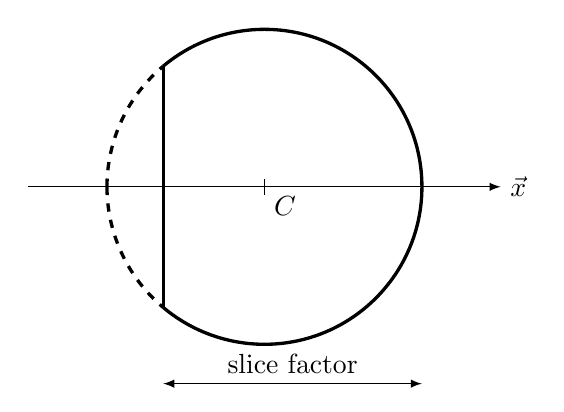
\begin{tikzpicture}
\draw [-latex] (-3,0) -- (3,0);
\draw (3,0) node[right]{$\vec{x}$};
\draw [-] (0,-0.1) -- (0,0.1);
\draw (0,0) node[below right]{$C$};

\draw [very thick,-](2,0) arc [start angle=0, end angle=130, radius=2];
\draw [very thick,-](2,0) arc [start angle=0, end angle=-130, radius=2];
\draw [very thick,dashed](-2,0) arc [start angle=180, end angle=130, radius=2];
\draw [very thick,dashed](-2,0) arc [start angle=180, end angle=230, radius=2];
\draw [very thick,-] (-1.2856,-1.5321) -- (-1.2856,1.5321);

\draw [latex-latex] (-1.2856,-2.5) -- (2,-2.5) node [midway,above] {slice factor};
\end{tikzpicture}\end{center}
There are two faces only to this object:
\begin{enumerate}
\setcounter{enumi}{-1}
	\item the spherical interface
	\item the flat face
\end{enumerate}
and two associated anchor points:
\begin{itemize}
	\item \textbf{SEL\_OBJ\_SPHERE\_CENTER}: the center of the sphere
	\item \textbf{SEL\_OBJ\_SPHERE\_SLICE\_CENTER}: the center of the flat face
\end{itemize}

\newpage
\subsection{Surface Primitives}

\subsubsection{Cylindrical surface}

\newpage
\subsubsection{Conical surface}

\newpage
\subsubsection{Disk}

Disks are flat surfaces that can help make diaphragms, and are added through \lfc{Selene\_object}(\lsg{disk},\lft{$r$},\lft{$r_{in}$}). The outer radius is defined by \lft{$r$}, and inner radius by \lft{$r_{in}$}. The disk extends in the $(y,z)$ plane, and its normal vector is pointed towards $-\vec x$.

Its only notable point is \textbf{SEL\_OBJ\_CENTER}.

\newpage
\subsubsection{Parabola}

Parabolas are basic optical surfaces that can be used to design aspheric lenses or parabolic mirrors. they can be added to a scene through \lfc{Selene\_object}(\lsg{parabola},\lft{focal},\lft{$r_{in}$},\lft{length}), with \lft{focal} the location of the focal point with respect to the apex and \lft{length} the total length of the parabola. The radius parameter \lft{$r_{in}$} is there to provide an easy way to open an aperture around the parabola tip.
\begin{center}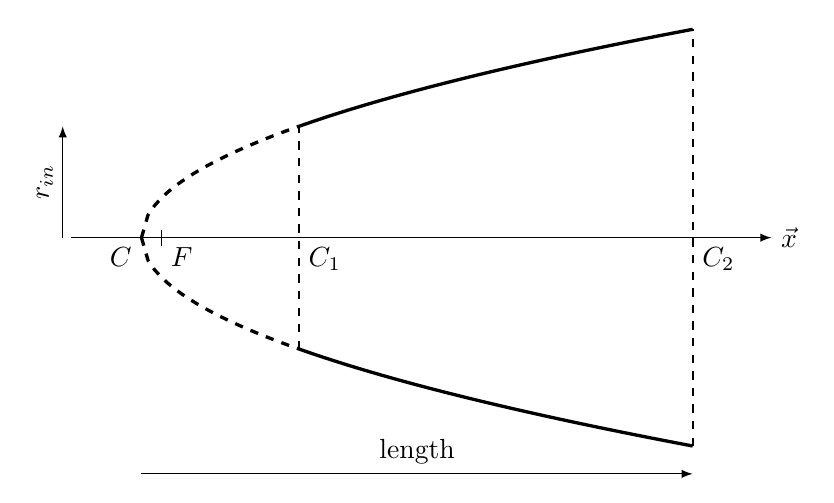
\begin{tikzpicture}
\draw [very thick,domain=0:2,dashed] plot (\x,{sqrt(\x)});
\draw [very thick,domain=2:7] plot (\x,{sqrt(\x)});
\draw [very thick,domain=0:2,dashed] plot (\x,{-sqrt(\x)});
\draw [very thick,domain=2:7] plot (\x,{-sqrt(\x)});
\draw [thick,dashed] (2,-1.4142) -- (2,1.4142);
\draw (2,0) node[below right]{$C_1$};
\draw [thick,dashed] (7,-2.6458) -- (7,2.6458);
\draw (7,0) node[below right]{$C_2$};
\draw [-] (-0.1,0) -- (0.1,0);
\draw (0,0) node[below left]{$C$};

\draw [-] (0.25,-0.1) -- (0.25,0.1);
\draw (0.25,0) node[below right]{$F$};

\draw [-latex] (-1,0) -- (-1,1.4142) node [midway,above,sloped] {$r_{in}$};

\draw [-latex] (0,-3) -- (7,-3) node [midway,above] {length};

\draw [-latex] (-0.9,0) -- (8,0);
\draw (8,0) node[right]{$\vec{x}$};
\end{tikzpicture}\end{center}
There is only one face to it, and its normal vector points outwards. There are, however, four notable points that can serve as anchors:
\begin{itemize}
	\item \textbf{SEL\_PARABOLA\_CENTER}: the tip of the parabola if it were full, noted by $C$ on the diagram above
	\item \textbf{SEL\_PARABOLA\_FOCUS}: the focal point of the parabola
	\item \textbf{SEL\_PARABOLA\_IN\_CENTER}: the center of the disk formed by the small aperture, noted $C_1$ above
	\item \textbf{SEL\_PARABOLA\_OUT\_CENTER}: the center of the disk formed by the end of the parabola, noted $C_2$ above
\end{itemize}

\newpage
\subsubsection{Rectangle}

The rectangle is the flat equivalent of the box. Is this created through \lfc{Selene\_object}(\lsg{rectangle},\lft{ly},\lft{lz}). It extends in the $(y,z)$ plane from -\lft{ly}/2 to +\lft{ly}/2, and -\lft{lz}/2 to +\lft{lz}/2.

The normal vector of the face is directed towards $-\vec x$. The only admissible anchor point is \textbf{SEL\_OBJ\_CENTER}.

\newpage
\subsubsection{Spherical patch}

\begin{itemize}
	\item \textbf{SEL\_OBJ\_SPHERE\_PATCH\_CENTER}
	\item \textbf{SEL\_OBJ\_SPHERE\_PATCH\_SLICE\_CENTER}
\end{itemize}

\subsection{Meshes}

This object type has access to specific functions
\begin{itemize}
	\item \lfc{add\_mesh}(\lsg{file\_name}): appends the mesh designed by \lsgnq{file\_name} to the object's mesh
	\item \lfc{auto\_recalc\_normals}(): recompute the face normals so that they all point outside
	\item \lfc{N\_faces}(): returns the total number of faces of the mesh
\end{itemize}

\subsubsection{Faces groups}

\lfc{define\_faces\_group}(\lin{group number},\lin{first face},\lin{last face})

\begin{itemize}
	\item \lfc{faces\_group\_down\_IRF}(\lin{group number},\lud{IRF})
	\item \lfc{faces\_group\_down\_mat}(\lin{group number},\lud{Material})
	\item \lfc{faces\_group\_down\_tangent}(\lin{group number},\lsg{type})
	\item \lfc{faces\_group\_down\_tangent}(\lin{group number},\lft{x},\lft{y},\lft{z})
	\item \lfc{faces\_group\_IRF}(\lin{group number},\lud{IRF})
	\item \lfc{faces\_group\_up\_IRF}(\lin{group number},\lud{IRF})
	\item \lfc{faces\_group\_up\_mat}(\lin{group number},\lud{Material})
	\item \lfc{faces\_group\_up\_tangent}(\lin{group number},\lsg{type})
	\item \lfc{faces\_group\_up\_tangent}(\lin{group number},\lft{x},\lft{y},\lft{z})
\end{itemize}

\subsection{Composite objects}

\subsubsection{Booleans}

\subsubsection{Composites}

\newpage
\section{Sensors}

\label{selene_sensors}
There would be not much point to a simulation software if one could do no analysis thanks to it. As such, some kind of sensors are necessary. In Selene, sensors are objects marked as such.

This is done through the \lfc{sensor} function, of which the first parameter specifies what kind of sensor. The following parameters specify what the sensor needs to record. Example:
\begin{lstlisting}
obj:sensor("abs","wavelength","ID","obj_intersection")
\end{lstlisting}

\subsection{Absorbing sensors}

This kind of sensor is basically a screen. Rays interacting with it are absorbed and disappear from the simulation. Absorbing sensors are specified with the \lsg{abs} parameter.

\subsection{Transparent sensors}

Object defined as transparent sensors behave according to their geometry, materials, IRFs, etc, but record interactions with rays. They can be used to monitor flux through a surface, or evaluate the number of rays that will be absorbed through a specific region of space. They are specified with the \lsg{transp} parameter.

\subsection{Recording options}

\begin{itemize}
	\item \lsg{wavelength}: records the ray wavelength
	\item \lsg{source}: records the ID of the source that generated the ray
	\item \lsg{path}: records the ray path ID. It is assigned by the source at generation, and can thus be common to several rays. It is unique for a single source.
	\item \lsg{generation}: records the ray number within a path, starting from 0, and increasing after each interaction
	\item \lsg{length}: records the ray optical path length at the intersection point
	\item \lsg{phase}: records the phase of the ray at the intersection point
	\item \lsg{world\_intersection}: records the coordinates of the intersection with respect to the scene frame
	\item \lsg{world\_direction}: records the directoin of the ray at the intersection with respect to the scene frame
	\item \lsg{obj\_intersection}: records the coordinates of the intersection with respect to the object frame
	\item \lsg{obj\_direction}: records the directoin of the ray at the intersection with respect to the object frame
\end{itemize}

\subsection{File format}

Objects marked as sensors will generate a file with a name like \lsgnq{object\_name\_ray\_sensor}.

The first line contains in the following order: the coordinates of the object center (three numbers), the vectors of the object frame (nine numbers), and the bounding box in the object frame. All those follow the $x$, $y$, $z$ order.

The second line is a string sequence that lists all the recorded options names.

Each subsequent line will correspond to an interaction containing the requested data in the order specified by the second line.

\newpage
\section{Sources}

Sources are what generate rays for the renderer to compute, and nothing would happen without them. They share many common functions with objects, but have a few dedicated ones. Source are created using the \lfc{Selene\_light}(\lsg{type},\lud{options...}) function. For instance
\begin{lstlisting}
light_1=Selene_light("point_planar")
\end{lstlisting}
will create a planar point source.

\subsection{Functions common to all light sources}

\label{selene_source_funcs}

\subsubsection[discrete\_spectrum]{\lfc{discrete\_spectrum}(\{\lft{lambda 1},\lft{lambda 2},\lft{...}\},\{\lft{weight 1},\lft{weight 2},\lft{...}\})}

Gives the source a discrete spectrum from a list of wavelength in meters, with their associated wavelengths
\begin{lstlisting}
light:discrete_spectrum({400e-9,500e-9,600e-9},{1,2,1.5})
\end{lstlisting}

\subsubsection[material]{\lfc{material}(\lud{Material})}

Sets the ambient material of the source to \lud{Material}.
\begin{lstlisting}
light:material(Glass)
\end{lstlisting}

\subsubsection[location]{\lfc{location}(\lft{x},\lft{y},\lft{z})}

Sets the source location to (\lft{x},\lft{y},\lft{z}) within the translation frame. The true location will be defined according to the relative positioning system. See \ref{selene_relative_positioning} for a detailled explanation.
\begin{lstlisting}
light:location(1,1,0)
\end{lstlisting}

\subsubsection[name]{\lfc{name}(\lsg{source name})}

Sets the source name to \lsgnq{name}.
\begin{lstlisting}
light:name("laser")
\end{lstlisting}

%\subsubsection[origin]{\lfc{origin}(\lsgnq{anchor name})}
%
%Sets the origin of the source to its anchor defined by \lsgnq{anchor name}. See \ref{selene_relative_positioning} for more details, and the sources descriptions for a list of the anchors.
%\begin{lstlisting}
%light:origin(SEL_LIGHT_BEAM_WAIST)
%\end{lstlisting}

\subsubsection[polar\_along]{\lfc{polar\_along}(\lft{x},\lft{y},\lft{z})}

Defines the axis vector (\lft{x},\lft{y},\lft{z}) along which the source will try to orient the polarization as close as possible. The sign of the whole vector is of no importance.
\begin{lstlisting}
light:polar_along(1,1,0)
\end{lstlisting}

\subsubsection[polar\_not]{\lfc{polar\_not}(\lft{x},\lft{y},\lft{z})}

Defines the axis vector (\lft{x},\lft{y},\lft{z}) that the source will try to avoid for rays polarization as much as possible. The sign of the whole vector is of no importance.
\begin{lstlisting}
light:polar_not(0,0,1)
\end{lstlisting}

\subsubsection[polar\_unset]{\lfc{polar\_unset}()}

Leaves to the source the choice of the polarization vector for each ray.
\begin{lstlisting}
light:polar_unset()
\end{lstlisting}

\subsubsection[power]{\lfc{power}(\lft{value})}

Sets the power of the source to anchor of the specified \lft{value} in Watts.
\begin{lstlisting}
light:power(55)
\end{lstlisting}

\subsubsection[relative\_origin]{\lfc{relative\_origin}(\lud{relative frame},\lsgnq{anchor name})}

Sets the relative origin of the source to anchor of the \lud{relative frame} designed by \lsgnq{anchor name}. See \ref{selene_relative_positioning} for more details, and the objects and sources descriptions for a list of the anchors.
\begin{lstlisting}
light:relative_origin(object_0,SEL_OBJ_BOX_FACE_XM)
\end{lstlisting}

\subsubsection[rotation]{\lfc{rotation}(\lft{$\alpha$},\lft{$\beta$},\lft{$\gamma$})}

Set the angles of rotation of the source to \lft{$\alpha$}, \lft{$\beta$} and \lft{$\gamma$}, in degrees, relative to the \lud{rotation frame}. See \ref{selene_relative_positioning} for more details.
\begin{lstlisting}
light:rotation(0,0,90)
\end{lstlisting}

\subsubsection[rotation\_frame]{\lfc{rotation\_frame}(\lud{frame})}

Set the relative rotation frame of the source the to one held by \lud{frame}. See \ref{selene_relative_positioning} for more details.
\begin{lstlisting}
light:rotation_frame(object_1)
\end{lstlisting}

\subsubsection[spectrum]{\lfc{spectrum}(\lsg{spectrum shape},\lud{option})}

Defines the source as a broadband source with the related \lsgnq{spectrum shape}. It can have three different values, with associated options.
\begin{itemize}
	\item \lfc{spectrum}(\lsg{flat},\lft{lambda min},\lft{lambda max}) will give the source a flat spectral flux between both boundaries, in meters
	\item \lfc{spectrum}(\lsg{file},\lsg{file\_name}) will load the associated file and assign it as the spectral flux of the source
	\item \lfc{spectrum}(\lsg{planck},\lft{lambda min},\lft{lambda max},\lft{temperature}) will define the source as a black body with the associated temperature in Kelvin, that will be sampled between the boundaries in meters
\end{itemize}

\subsubsection[translation\_frame]{\lfc{translation\_frame}(\lud{frame})}

Set the relative translation frame of the source to the one held by \lud{frame}. See \ref{selene_relative_positioning} for more details.
\begin{lstlisting}
light:translation_frame(lens)
\end{lstlisting}

\subsubsection[wavelength]{\lfc{wavelength}(\lft{lambda})}

Defines the source as a monochromatic source of wavelength \lft{lambda}, in meters.
\begin{lstlisting}
light:wavelength(533e-9)
\end{lstlisting}

\subsection{Source types}

\subsubsection{Perfect beam}

This source aims to represent a source place at infinity. Its rays are strictly parallel, along the $x$ axis of the source. It is instanced by the \lsg{perfect\_beam} parameter.

The function \lfc{aperture}(\lft{radius}) will set the size of the disk emitting the rays with the corresponding \lft{radius}, in meters.

\noindent Example:
\begin{lstlisting}
light=Selene_light("perfect_beam")
light:aperture(5e-3)
\end{lstlisting}

\subsubsection{Planar point source}

This source is similar to the point source, except it will emit in its $(y,z)$ plane only. A rotation by $\gamma=90^\circ$ is thus necessary to target the $(x,y)$ plane. It is created through the \lsg{point\_planar} parameter.\\ Example:
\begin{lstlisting}
light=Selene_light("point_planar")
\end{lstlisting}

\subsubsection{Point source}

This is the most basic source. It will emit in all directions homogeneously. It is created through the \lsg{point} parameter.\\ Example:
\begin{lstlisting}
light=Selene_light("point")
\end{lstlisting}

\subsection{Spectra}

To different types of analysis will correspond different input spectra. We provide a few ways of handling them.

In order to easily match the CIE illuminants, we assume all the spectra are actually spectral power distributions, in $W\cdot m^{-1}$, although this does not define the actual power of the source.

\subsubsection{Monochromatic sources}

Those are the most basic types of spectra. Every ray generated by those sources will be assigned the wavelength defined by \lfc{wavelength}.

\subsubsection{Poly-monochromatic sources}

They are the bridge between monochromatic sources and truly polychromatic sources, and can approximate lights with a small number of emission rays.

They are basically several monochromatic sources bundled into one, but with different weights associated with each wavelengths. Those wavelengths are then probabilistically given to the generated rays according to those weights.

Such spectra are assigned through the \lfc{discrete\_spectrum} function.

\subsubsection{Polychromatic sources}

Those are the truly polychromatic sources. In this, the spectrum is a continuous function going from $\lambda_{min}$ to $\lambda_{max}$. Wavelengths are then assigned to generated rays thanks to a rejection algorithm between those boundaries. We provide three types of polychromatic spectra
\begin{description}
	\item[Flat]: every wavelength between $\lambda_{min}$ and $\lambda_{max}$ is equiprobable
	\item[Planck]: the probability distribution here is the black body distribution in wavelength form
	\begin{equation}
		P(\lambda,T)=\frac{2*h*c^3}{\lambda^5}\frac{1}{e^{\dse -\frac{hc}{\lambda k_B T}}-1}
	\end{equation}
	\item[User defined]: in this case, the user provides a two columns text file, the first being the wavelength, and the second the associated probability. Wavelengths are then drawn to match this probability distribution
\end{description}

\subsection{Power normalization, spectra and rays}

\subsubsection{Time}

Time is an undefined quantity with respect to raytracing. One can could assume all the paths are computed exactly at the same time, or spread across several seconds. For convenience, it was decided computations would occur within one second, so that the values of power and total energy emitted could be treated as the same.

\subsubsection{Energy}

Generally, rays can not represent real photons due to the sheer number of those cast by a real light source. For instance, a 1W source would emit in the order of $10^{20}$ photons per second, and computing them all would require incredible computational power.

The issue is then figuring out how to represent those photons with far fewer of them, in particular the energy they carry. Real photons energy is wavelength dependent, with $E=hc/\lambda$, but using this is not particularly convenient.

For instance, let us assume we want to simulate a light source with a flat power spectrum: using the previous definition would imply that for one blue ray emitted by the source, there would be two red ones. Since the computation spatial accuracy is a factor of the number of rays cast, it would be twice as good for red ones than blue ones, which is leads to an imbalance in simulation results.

As such, it was decided that, by default, all rays should carry the same number amount of energy.

\subsubsection{Number of rays per source}

The total number of photons is set by the user, and they need to be distributed among sources. This is done thanks to the \lfc{power} function which is serves both to relate sources to eachother, and to define how much energy rays will carry.

If each source $i$ emits a power $P_i$, and the total number of photons is $N$, then the number of rays per source $N_i$ will be
\begin{equation}
	N_i=N\frac{P_i}{\dse \sum_i P_i}
\end{equation}
and the power of each ray will be
\begin{equation}
	P_r=\frac{1}{N} \sum_i P_i
\end{equation}